%! TeX root = ../../main.tex

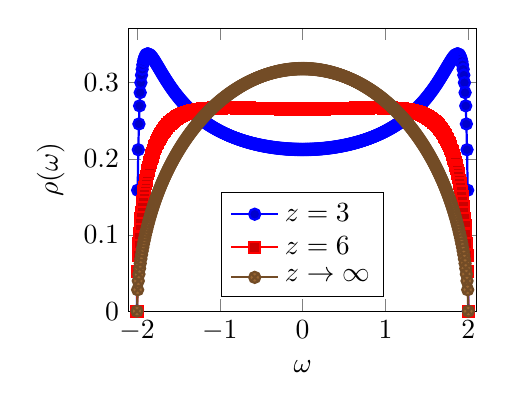
\begin{tikzpicture}
    \begin{axis}
        [
            width=6cm,
            xlabel=$\omega$,
            ylabel=$\rho(\omega)$,
            xmin=-2.1,
            xmax=2.1,
            ymin=0,
            every axis plot/.append style=
                {
                    thick,
                    domain=-2:2,
                    samples=513, % 2^n + 1 to ensure inclusion of last point
                },
            legend cell align=left,
            legend entries={
                    $z=3$,
                    $z=6$,
                    $z\rightarrow\infty$,
                },
            legend style={
                    at={(0.5, 0.05)},
                    anchor=south,
                },
        ]

        \addplot {1/(2*pi) * sqrt(4 - x^2) / (3/(3-1) - x^2/3}; % z=3
        \addplot {1/(2*pi) * sqrt(4 - x^2) / (6/(6-1) - x^2/6}; % z=6
        \addplot {1/(2*pi) * sqrt(4 - x^2)}; % z\to\infty
    \end{axis}
\end{tikzpicture}
